\chapter{Membangun Model Prediksi}
\section{Teori}
\subsection{Binary Classification}
\begin{enumerate}
\item Binary classification yaitu berupa kelas positif dan kelas negatif. Klasifikasi biner adalah dikotomisasi yang diterapkan untuk tujuan praktis, dan dalam banyak masalah klasifikasi biner praktis, kedua kelompok tidak simetris - daripada akurasi keseluruhan, proporsi relatif dari berbagai jenis kesalahan yang menarik. Misalnya, dalam pengujian medis, false positive (mendeteksi penyakit ketika tidak ada) dianggap berbeda dari false negative (tidak mendeteksi penyakit ketika hadir).
\begin{figure}[ht]
\centering
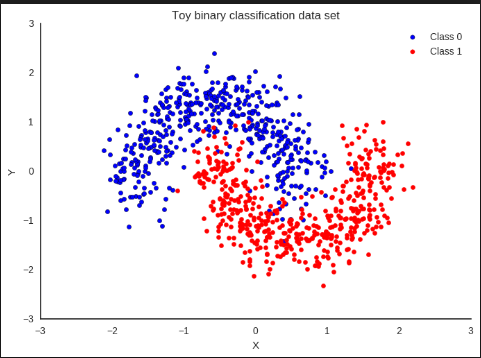
\includegraphics[scale=0.5]{figures/wiendh1.png}
\caption{Binary Classification}
\label{contoh}
\end{figure}
\end{enumerate}

\subsection{Supervised Learning, Unsupervised Learning dan Clustering }
\begin{enumerate}
\item Supervised learning adalah tugas pembelajaran mesin untuk mempelajari suatu fungsi yang memetakan input ke output berdasarkan contoh pasangan input-output. Ini menyimpulkan fungsi dari data pelatihan berlabel yang terdiri dari serangkaian contoh pelatihan. Dalam pembelajaran yang diawasi, setiap contoh adalah pasangan yang terdiri dari objek input (biasanya vektor) dan nilai output yang diinginkan (juga disebut sinyal pengawas). Algoritma pembelajaran yang diawasi menganalisis data pelatihan dan menghasilkan fungsi yang disimpulkan, yang dapat digunakan untuk memetakan contoh-contoh baru. Skenario optimal akan memungkinkan algoritma menentukan label kelas dengan benar untuk instance yang tidak terlihat. Ini membutuhkan algoritma pembelajaran untuk menggeneralisasi dari data pelatihan untuk situasi yang tidak terlihat dengan cara yang "masuk akal" (lihat bias induktif). Tugas paralel dalam psikologi manusia dan hewan sering disebut sebagai pembelajaran konsep. Contoh dibawah yaitu Supervised Learning dengan SVC.
\begin{figure}[ht]
\centering
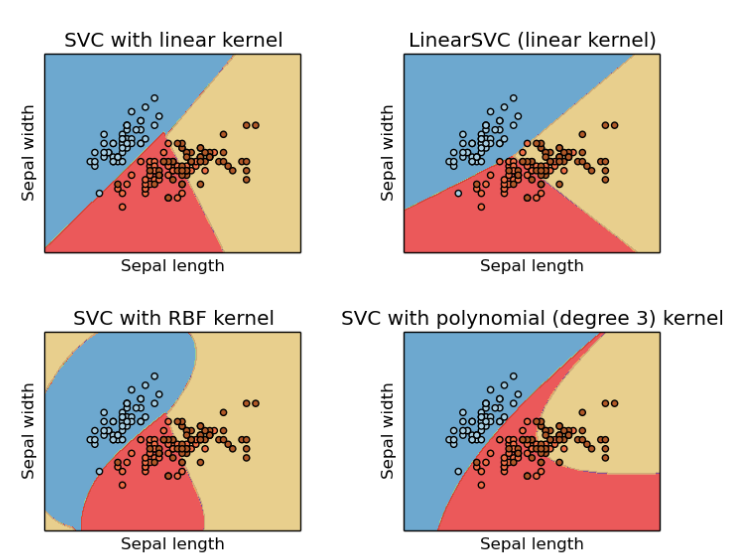
\includegraphics[scale=0.5]{figures/wiendh2.png}
\caption{Supervised Learning}
\label{contoh}
\end{figure}
\item Unsupervised learning adalah istilah yang digunakan untuk pembelajaran bahasa Ibrani, yang terkait dengan pembelajaran tanpa guru, juga dikenal sebagai organisasi mandiri dan metode pemodelan kepadatan probabilitas input. Analisis cluster sebagai cabang pembelajaran mesin yang mengelompokkan data yang belum diberi label, diklasifikasikan atau dikategorikan. Alih-alih menanggapi umpan balik, analisis klaster mengidentifikasi kesamaan dalam data dan bereaksi berdasarkan ada tidaknya kesamaan di setiap potongan data baru. BErikut merupakan contoh Unsupervised Learning dengan Gaussian mixture models.
\begin{figure}[ht]
\centering
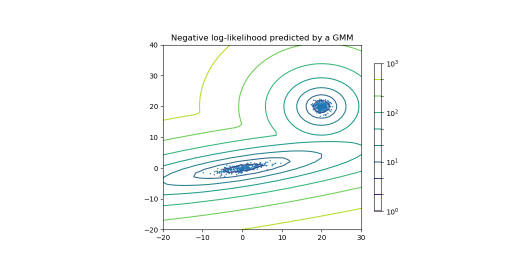
\includegraphics[scale=0.5]{figures/wiendh3.png}
\caption{Unsupervised Learning}
\label{contoh}
\end{figure}
\item Cluster analysis or clustering adalah tugas pengelompokan sekumpulan objek sedemikian rupa sehingga objek dalam kelompok yang sama (disebut klaster) lebih mirip (dalam beberapa hal) satu sama lain daripada pada kelompok lain (kluster). Ini adalah tugas utama penambangan data eksplorasi, dan teknik umum untuk analisis data statistik, yang digunakan di banyak bidang, termasuk pembelajaran mesin, pengenalan pola, analisis gambar, pengambilan informasi, bioinformatika, kompresi data, dan grafik komputer. Analisis Cluster sendiri bukan merupakan salah satu algoritma spesifik, tetapi tugas umum yang harus dipecahkan. Ini dapat dicapai dengan berbagai algoritma yang berbeda secara signifikan dalam pemahaman mereka tentang apa yang merupakan sebuah cluster dan bagaimana cara menemukannya secara efisien. Gagasan populer mengenai cluster termasuk kelompok dengan jarak kecil antara anggota cluster, area padat ruang data, interval atau distribusi statistik tertentu. Clustering karena itu dapat dirumuskan sebagai masalah optimasi multi-objektif. Algoritma pengelompokan dan pengaturan parameter yang sesuai (termasuk parameter seperti fungsi jarak yang akan digunakan, ambang kepadatan atau jumlah cluster yang diharapkan) tergantung pada set data individual dan penggunaan hasil yang dimaksudkan. Analisis kluster bukan merupakan tugas otomatis, tetapi proses berulang penemuan pengetahuan atau optimasi multi-objektif interaktif yang melibatkan percobaan dan kegagalan. Seringkali diperlukan untuk memodifikasi praproses data dan parameter model hingga hasilnya mencapai properti yang diinginkan.
\begin{figure}[ht]
\centering
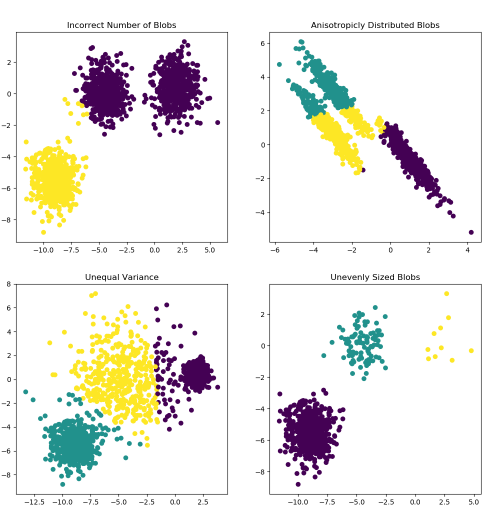
\includegraphics[scale=0.5]{figures/wiendh4.png}
\caption{Cluster}
\label{contoh}
\end{figure}
\end{enumerate}

\subsection{Evaluasi dan Akurasi}
\begin{enumerate}
\item Evaluasi adalah tentang  bagaimana kita dapat mengevaluasi seberapa baik model bekerja dengan mengukur akurasinya. Dan akurasi akan didefinisikan sebagai persentase kasus yang diklasifikasikan dengan benar. Kita dapat menganalisis kesalahan yang dibuat oleh model, atau tingkat kebingungannya, menggunakan matriks kebingungan. Matriks kebingungan mengacu pada kebingungan dalam model, tetapi matriks kebingungan ini bisa menjadi sedikit sulit untuk dipahami ketika mereka menjadi sangat besar.
\begin{figure}[ht]
\centering
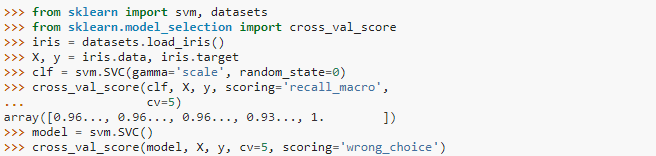
\includegraphics[scale=0.5]{figures/wiendh9.png}
\caption{ Evaluasi dan Akurasi}
\label{contoh}
\end{figure}
\end{enumerate}

\subsection{ Cara membuat dan membaca confusion matrix }
\begin{enumerate}
\item Cara membuat dan membaca confusion matrix :
\begin{itemize}
\item 1)	Tentukan pokok permasalahan dan atributanya, misal gaji dan listik.
\item 2)	Buat pohon keputusan
\item 3)	Lalu data testingnya
\item 4)	Lalu mencari nilai a, b, c, dan d. Semisal a = 5, b = 1, c = 1, dan d = 3.
\item 5)	Selanjutnya mencari nilai recall, precision, accuracy, serta dan error rate.
\end{itemize}
\item Berikut adalah contoh dari confusion matrix :
\begin{itemize}
\item Recall =3/(1+3) = 0,75
\item Precision = 3/(1+3) = 0,75
\item Accuracy =(5+3)/(5+1+1+3) = 0,8
\item Error Rate =(1+1)/(5+1+1+3) = 0,2
\end{itemize}
\end{enumerate}

\subsection{K-fold cross validation}
\begin{enumerate}
\item Cara kerja K-fold cross validation :
\begin{itemize}
\item 1)	Total instance dibagi menjadi N bagian.
\item 2)	Fold yang pertama adalah bagian pertama menjadi data uji (testing data) dan sisanya menjadi training data.
\item 3)	Lalu hitung akurasi berdasarkan porsi data tersebut dengan menggunakan persamaan.
\item 4)	Fold yang ke dua adalah bagian ke dua menjadi data uji (testing data) dan sisanya training data. 
\item 5)	Kemudian hitung akurasi berdasarkan porsi data tersebut.
\item 6)	Dan seterusnya hingga habis mencapai fold ke-K.
\item 7)	Terakhir hitung rata-rata akurasi K buah.
\end{itemize}
\begin{figure}[ht]
\centering
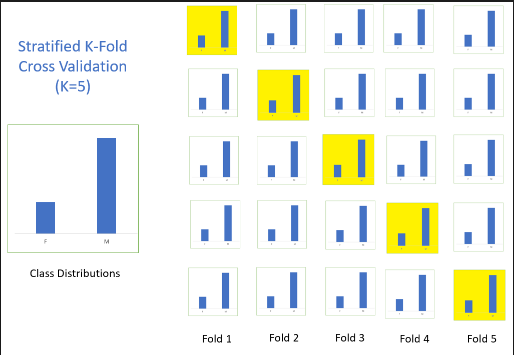
\includegraphics[scale=0.5]{figures/wiendh5.png}
\caption{K-fold cross validation }
\label{contoh}
\end{figure}
\end{enumerate}

\subsection{Decision Tree }
\begin{enumerate}
\item Decision Tree dalah metode pembelajaran yang diawasi non-parametrik yang digunakan untuk klasifikasi dan regresi. Tujuannya adalah untuk membuat model yang memprediksi nilai variabel target dengan mempelajari aturan keputusan sederhana yang disimpulkan dari fitur data.\\
Misalnya, dalam contoh di bawah ini, decision tree belajar dari data untuk memperkirakan kurva sinus dengan seperangkat aturan keputusan if-then-else. Semakin dalam pohon, semakin rumit aturan keputusan dan semakin bugar modelnya.
\begin{figure}[ht]
\centering
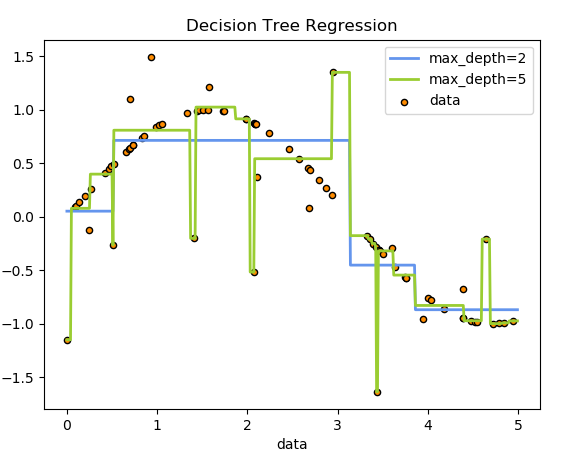
\includegraphics[scale=0.5]{figures/wiendh6.png}
\caption{Decision Tree}
\label{contoh}
\end{figure}
\end{enumerate}

\subsection{Information Gain dan Entropi}
\begin{enumerate}
\item Information gain didasarkan pada penurunan entropi setelah dataset dibagi pada atribut. Membangun decision tree adalah semua tentang menemukan atribut yang mengembalikan perolehan informasi tertinggi (mis., Cabang yang paling homogen).
\begin{figure}[ht]
\centering
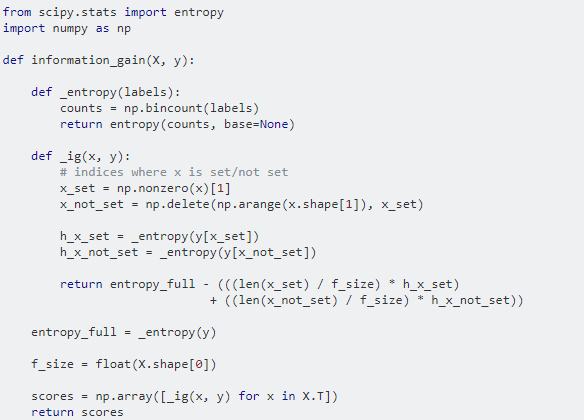
\includegraphics[scale=0.5]{figures/wiendh7.png}
\caption{Information gain}
\label{contoh}
\end{figure}
\item Entropi adalah ukuran keacakan dalam informasi yang sedang diproses. Semakin tinggi entropi, semakin sulit untuk menarik kesimpulan dari informasi itu. Membalik koin adalah contoh tindakan yang memberikan informasi yang acak. Untuk koin yang tidak memiliki afinitas untuk kepala atau ekor, hasil dari sejumlah lemparan sulit diprediksi. Mengapa? Karena tidak ada hubungan antara membalik dan hasilnya. Inilah inti dari entropi.
\begin{figure}[ht]
\centering
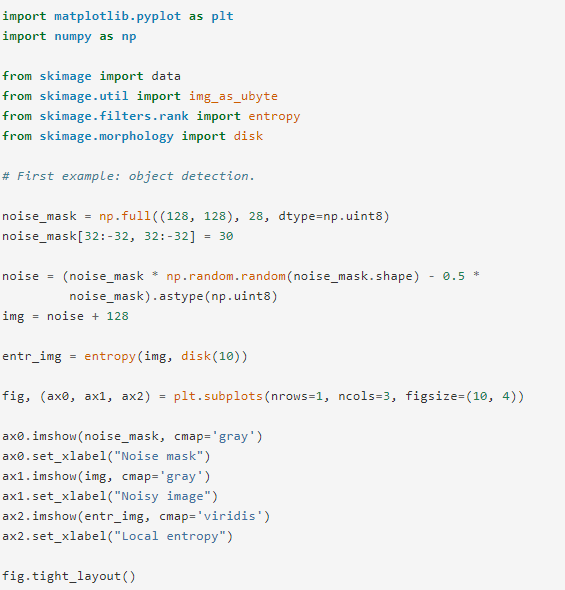
\includegraphics[scale=0.5]{figures/wiendh8.png}
\caption{Entropi}
\label{contoh}
\end{figure}
\end{enumerate}

\section{Pratikum}
\subsection{Scikit-Learn}
\begin{enumerate}

\item
\begin{verbatim}
	# load dataset (student mat pakenya)
	import pandas as pd
	durian = pd.read_csv('student-mat.csv', sep=';')
	len(d)
\end{verbatim}

\par
Codingan diatas digunakan untuk mengimport atau memanggil module pandas sebagai pd. Kemudian mendefinisikan variabel "durian" yang akan memanggil dataset yang didapatkan dari data csv. Jika skrip dijalankan di Spyder, hasilnya seperti berikut 
\begin{figure}[ht]
\centering
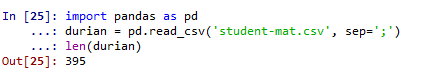
\includegraphics[scale=0.5]{figures/spyder1.png}
\caption{Loading Dataset}
\label{Spyder}
\end{figure}
\item
\begin{verbatim}
	# generate binary label (pass/fail) based on G1+G2+G3 
	# (test grades, each 0-20 pts); threshold for passing is sum>=30
	durian['pass'] = durian.apply(lambda row: 1 if (row['G1']+row['G2']+row['G3']) 
											>= 35 else 0, axis=1)
	durian = durian.drop(['G1', 'G2', 'G3'], axis=1)
	durian.head()
\end{verbatim}

\par
ada bagian ini mendeklarasikan pass/fail nya data berdasarkan G1+G2+G3. Dengan ketentuan nilai pass nya yaitu sama dengan 30.
kemudian pada variabel durian dideklarasikan  jika baris dengan G1+G2+G3 ditambahkan, dan hasilnya sama dengan 35 maka axisnya 1. ketika dijalankan hasilnya seperti berikut
\begin{figure}[ht]
\centering
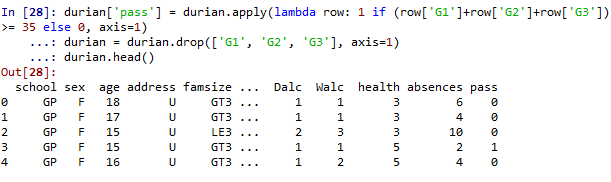
\includegraphics[scale=0.5]{figures/spyder2.png}
\caption{Generate Binary Label}
\label{Spyder}
\end{figure}
\item
\begin{verbatim}
	# use one-hot encoding on categorical columns
	durian = pd.get_dummies(durian, columns=['sex', 'school', 'address', 
									'famsize', 
									'Pstatus', 'Mjob', 'Fjob', 
	                               'reason', 'guardian', 'schoolsup', 
								   'famsup', 'paid', 'activities',
	                               'nursery', 'higher', 'internet', 
									'romantic'])
	durian.head()
\end{verbatim}
\par
One-hot encoding adalah proses di mana variabel kategorikal dikonversi menjadi bentuk yang dapat disediakan untuk algoritma ML untuk melakukan pekerjaan yang lebih baik dalam prediksi. Karena saya memuat data menggunakan panda, disini menggunakan fungsi panda pdgetdummies untuk jenis kelamin , sekolah, alamat dll. Metode head ini digunakan untuk mengembalikan baris n atas 5 secara default dari frame atau seri data. hasilnya seperti berikut 
\begin{figure}[ht]
\centering
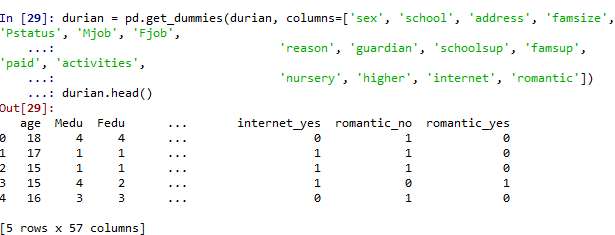
\includegraphics[scale=0.5]{figures/spyder3.png}
\caption{One-hot Encoding}
\label{Spyder}
\end{figure}
\item
\begin{verbatim}
	# shuffle rows
	durian = durian.sample(frac=1)
	# split training and testing data
	durian_train = d[:500]
	durian_test = d[500:]

	durian_train_att = durian_train.drop(['pass'], axis=1)
	durian_train_pass = durian_train['pass']

	durian_test_att = durian_test.drop(['pass'], axis=1)
	durian_test_pass = durian_test['pass']

	durian_att = durian.drop(['pass'], axis=1)
	durian_pass = d['pass']

	# number of passing students in whole dataset:
	import numpy as np
	print("Passing: %d out of %d (%.2f%%)" % (np.sum(d_pass), len(d_pass), 
	       100*float(np.sum(d_pass)) / len(d_pass)))
\end{verbatim}

\par
Sammple digunakan untuk mengembalikan sampel acak item dari objek. Pada bagian tersebut, terdapat train dan test yaing digunakan untuk untuk membagi train, test dan kemudian membagi lagi train ke validasi dan test.\\
Kemudia akan mengimport module numpy sebagai np yang akan digunakan untuk mengembalikan nilai passing dari pelajar dari keseluruhan dataset dengan cara print.
\begin{figure}[ht]
\centering
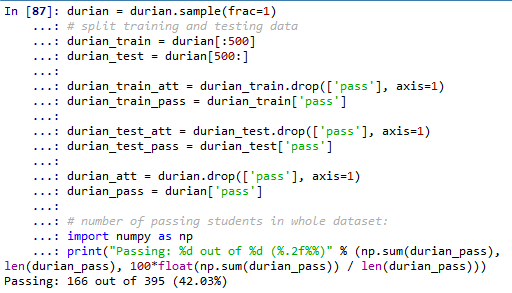
\includegraphics[scale=0.5]{figures/spyder4.png}
\caption{Shuffle Rows}
\label{Spyder}
\end{figure}
\item 
\begin{verbatim}
	# fit a decision tree
	from sklearn import tree
	mangga = tree.DecisionTreeClassifier(criterion="entropy", max_depth=5)
	mangga = mangga.fit(durian_train_att, durian_train_pass)
\end{verbatim}

\par
Dari librari scikitlearn import modul tree. Kemudian definisikan variabel Mangga dengan menggunakan DecisionClassifier. KEmudian pada variabel mangga terdapat Criterion yaitu suatu fungsi untuk mengukur kualitas split, setelah itu agar DecisionTreeClassifier dapat dijalankan gunakan perintah fit. hasilnya seperti dibawah
\begin{figure}[ht]
\centering
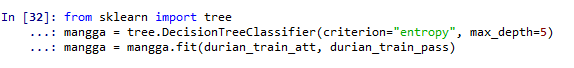
\includegraphics[scale=0.5]{figures/spyder5.png}
\caption{Fit Decision Tree}
\label{Spyder}
\end{figure}
\item
\begin{verbatim}
	# visualize tree
	import graphviz
	dot_data = tree.export_graphviz(mangga, out_file=None, label="all", 
									impurity=False, proportion=True,
	                                feature_names=list(durian_train_att), 
									class_names=["fail", "pass"], 
	                                filled=True, rounded=True)
	graph = graphviz.Source(dot_data)
	graph
\end{verbatim}

\par
Graphviz adalah perangkat lunak visualisasi grafik open source. Visualisasi grafik adalah cara mewakili informasi struktural sebagai diagram grafik dan jaringan abstrak. TREEEXPORTGRAPHVIZ merupakan fungsi yang menghasilkan representasi Graphviz dari decision tree, yang kemudian ditulis ke outfile. Sehingga akan muncul gambardiagram  grafik bercabang.
\begin{figure}[ht]
\centering
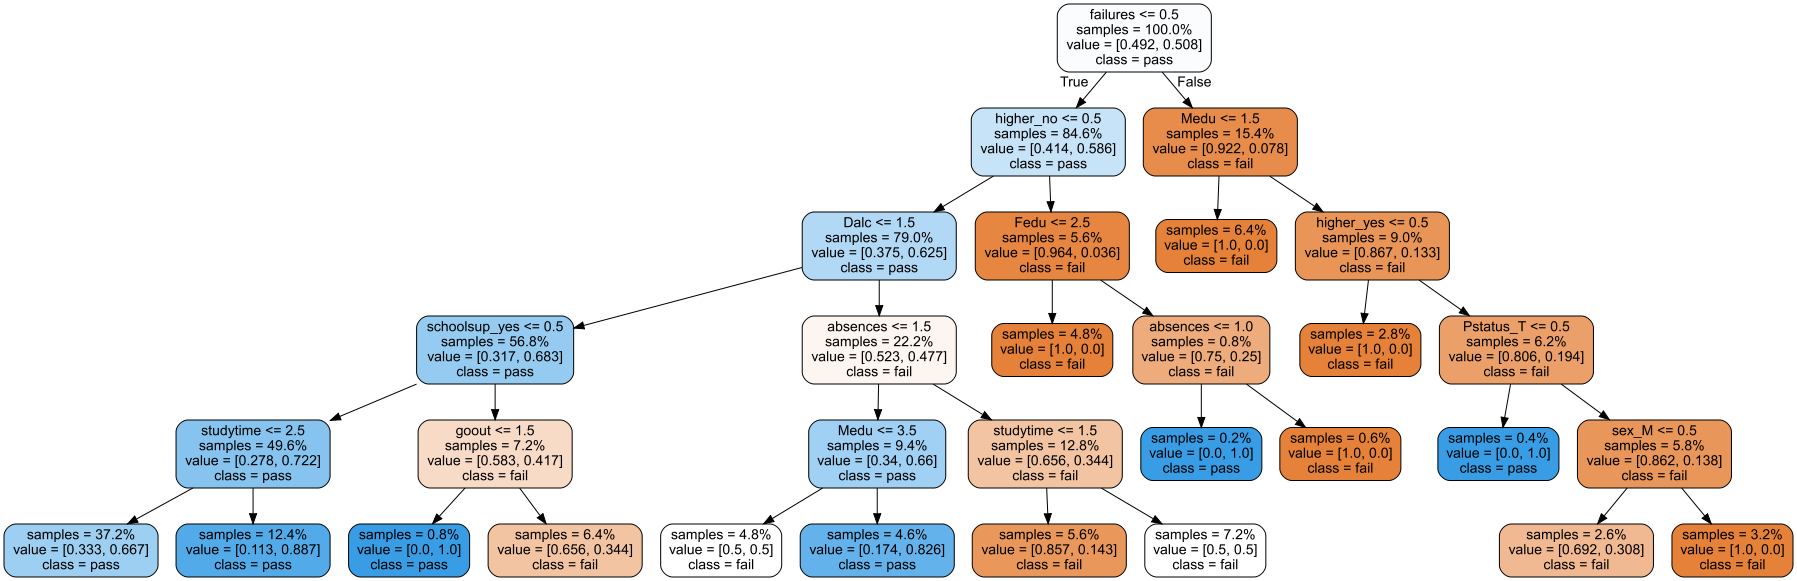
\includegraphics[scale=0.5]{figures/spyder6.png}
\caption{Fit Decision Tree}
\label{Spyder}
\end{figure}
\item
\begin{verbatim}
	# save tree
	tree.export_graphviz(mangga, out_file="student-performance.dot", 
						 label="all", impurity=False, 
						 proportion=True,
	                     feature_names=list(durian_train_att), 
	                     class_names=["fail", "pass"], 
	                     filled=True, rounded=True)
\end{verbatim}

\par
TREEEXPORTGRAPHVIZ merupakan fungsi yang menghasilkan representasi Graphviz dari decision tree, yang kemudian ditulis ke outfile.Disini akan menyimpan classifiernya, akan meng ekspor file student performance jika salah akan mengembalikan nilai fail.
\begin{figure}[ht]
\centering
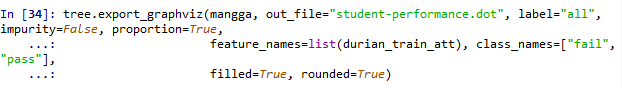
\includegraphics[scale=0.5]{figures/spyder7.png}
\caption{Fit Decision Tree}
\label{Spyder}
\end{figure}
\item
\begin{verbatim}
	mangga.score(durian_test_att, durian_test_pass)
\end{verbatim}

\par
Score juga disebut prediksi, dan merupakan proses menghasilkan nilai berdasarkan model pembelajaran mesin yang terlatih, diberi beberapa data input baru. Nilai atau skor yang dibuat dapat mewakili prediksi nilai masa depan, tetapi mereka juga mungkin mewakili kategori atau hasil yang mungkin. Jadi disini Mangga akan memprediksi nilai dari durian test att dan test pass. Hasilnya seperti dibawah ini
\begin{figure}[ht]
\centering
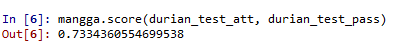
\includegraphics[scale=0.5]{figures/spyder8.png}
\caption{Score}
\label{Spyder}
\end{figure}
\item
\begin{verbatim}
	from sklearn.model_selection import cross_val_score
	nangka = cross_val_score(mangga, durian_att, durian_pass, cv=5)
	# show average score and +/- two standard deviations away 
	#(covering 95% of scores)
	print("Accuracy: %0.2f (+/- %0.2f)" % (nangka.mean(), nangka.std() * 2))
\end{verbatim}

\par
Skrip ini akan mengevaluasi score dengan validasi silang. Dimana variabel nangka berisikan crossvalscore yang merupakan fungsi pembantu pada estimator dan dataset. Kemudian akan menampilkan score rata rata dan kurang lebih dua standar deviasi yang mencakup 95 persen score. dengan menggunakan perintah print hasil yang didapatkan sebagai berikut
\begin{figure}[ht]
\centering
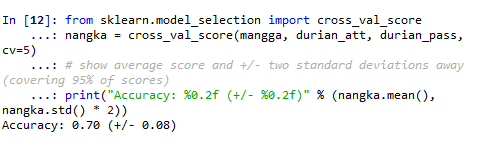
\includegraphics[scale=0.5]{figures/spyder9.png}
\caption{Cross Val Score}
\label{Spyder}
\end{figure}
\item 
\begin{verbatim}
	for max_depth in range(1, 20):
	    mangga = tree.DecisionTreeClassifier(criterion="entropy", 
			max_depth=max_depth)
	    nangka = cross_val_score(mangga, durian_att, durian_pass, cv=5)
	    print("Max depth: %d, Accuracy: %0.2f (+/- %0.2f)" % 
				(max_depth, nangka.mean(), nangka.std() * 2)
			 )
\end{verbatim}

\par
Pada skrip ini menunjukkan seberapa dalam tree itu. Semakin dalam tree, semakin banyak perpecahan yang dimilikinya dan menangkap lebih banyak informasi tentang data. variabel mangga akan mendefinisikan tree nya yang kemudian variabel nangka akan mengevaluasi score dengan validasi silang. disini mendefinisikan decision tree dengan kedalaman mulai dari 1 hingga 20 dan merencanakan pelatihan dan menguji skor auc. Jika di run hasilnya seperti berikut
\begin{figure}[ht]
\centering
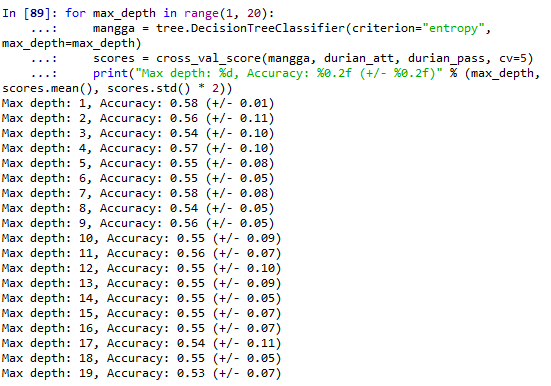
\includegraphics[scale=0.5]{figures/spyder10.png}
\caption{Max Depth}
\label{Spyder}
\end{figure}
\item
\begin{verbatim}
	depth_acc = np.empty((19,3), float)
	i = 0
	for max_depth in range(1, 20):
	    mangga = tree.DecisionTreeClassifier(criterion="entropy", 
			max_depth=max_depth)
	    nangka = cross_val_score(t, d_att, d_pass, cv=5)
	    depth_acc[i,0] = max_depth
	    depth_acc[i,1] = nangka.mean()
	    depth_acc[i,2] = nangka.std() * 2
	    i += 1

	depth_acc
\end{verbatim}

\par
Depth acc akan membuat array kosong dengan mengembalikan array baru dengan bentuk dan tipe yang diberikan, tanpa menginisialisasi entri. Dengan 19 sebagai bentuk array kosong, 3 sebagai output data-type dan float urutan kolom-utama (gaya Fortran) dalam memori. variabel mangga yang akan melakukan split score dan nangka akan mengvalidasi score secara silang. dan pada akhirnya nangka std yaitu menghitung standar deviasi dari data yang diberikan (elemen array) di sepanjang sumbu yang ditentukan (jika ada), hasilnya sebagai berikut
\begin{figure}[ht]
\centering
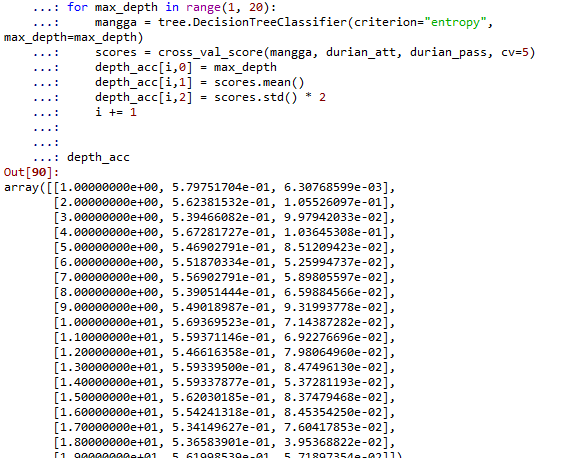
\includegraphics[scale=0.5]{figures/spyder11.png}
\caption{Depth in Range}
\label{Spyder}
\end{figure}
\item 
\begin{verbatim}
	import matplotlib.pyplot as plt
	fig, ax = plt.subplots()
	ax.errorbar(depth_acc[:,0], depth_acc[:,1], yerr=depth_acc[:,2])
	plt.show()
\end{verbatim}

\par
Mengimpor librari dari matplotlib yaitu pylot sebagai plt
fig dan ax menggunakan subplots untuk membuat gambar dan satu set subplot.
axerrorbar akan membuat error bar
kemudian grafik akan ditampilkan menggunakan show. Grafiknya seperti berikut

\begin{figure}[ht]
\centering
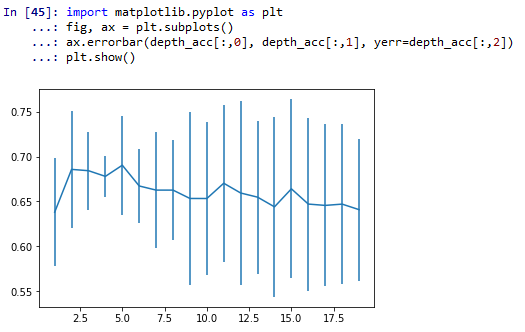
\includegraphics[scale=0.5]{figures/spyder12.png}
\caption{Matplotlib}
\label{Spyder}
\end{figure}
\end{enumerate}


\subsection{Penanganan Error}
\subsubsection{Error Graphviz}
\begin{enumerate}
	\item
Berikut ini merupakan eror yang didapatkan saat menjalankan graphviz pada Spyder
\begin{figure}[ht]
\centering
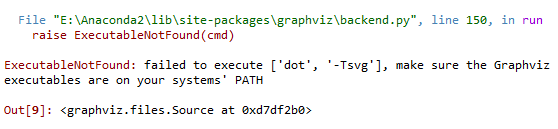
\includegraphics[scale=0.5]{figures/erorspyder1.png}
\caption{Error Graphviz}
\label{Error}
\end{figure}
	\item
Pada gambar diatas kode erornya adalah ExecutableNotFound failed to execute dot Tsvg. Eror ini terjadi karena tidak terdaftarnya environment variable dari Graphviz pada PATH di PC.
	\item
Solusi yang bisa dilakukan untuk mengatasi eror tersebut adalah sebagai berikut : \\
\begin{itemize}
\item
Buka Folder dimana Anaconda2 terinstall. Disini Anacondanya terinstal di folder E
\item
Kemudian, pada Anaconda2 buka Library/Bin/graphviz
\begin{figure}[ht]
\centering
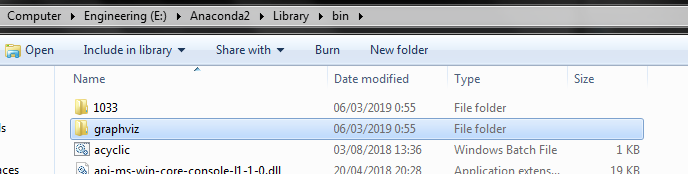
\includegraphics[scale=0.5]{figures/solusi3.png}
\caption{Folder Graphviz}
\label{Eror}
\end{figure}
\item
Salin alamat tersebut, kemudian buka Environment Variable dan Edit. 
\item
Pada bagian PATH pilih edit, dan salin alamat tersebut seperti berikut :
\begin{figure}[ht]
\centering
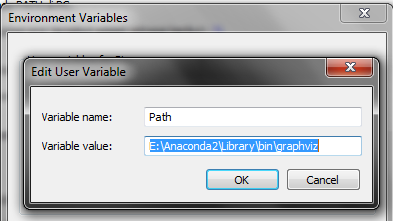
\includegraphics[scale=0.5]{figures/solusi4.png}
\caption{Menambahkan Graphviz kePATH}
\label{Eror}
\end{figure}
\item
Klik ok, kemudian restart Spyder dan jalankan kembali Skrip, maka hasilnya akan seperti berikut dan eror berhasil diselesaikan
\begin{figure}[ht]
\centering
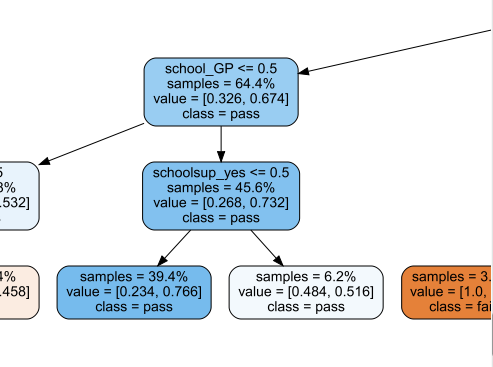
\includegraphics[scale=0.5]{figures/solusi5.png}
\caption{Evaluasi Eror}
\label{Eror}
\end{figure}
\end{itemize}
\end{enumerate}

\subsubsection{Error File Not Exist}
\begin{enumerate}
	\item
Berikut ini merupakan eror yang didapatkan saat menjalankan file csv sebagai dataset
\begin{figure}[ht]
\centering
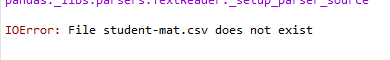
\includegraphics[scale=0.5]{figures/erorspyder2.png}
\caption{Error File Not Exist}
\label{Error}
\end{figure}
	\item
Pada gambar diatas kode erornya adalah IOError File student csv does not exist. Eror ini terjadi karena file yang dituju tidak berada didalam file yang salam dengan skrip ataupun filenya belum didefinisikan.
	\item
Solusi yang bisa dilakukan untuk mengatasi eror tersebut adalah sebagai berikut : \\
\begin{itemize}
\item
Buka Spyder, kemudian pada pojok kanan atas ada kolom sebagai berikut
\begin{figure}[ht]
\centering
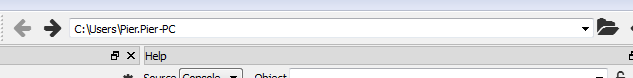
\includegraphics[scale=0.5]{figures/solusi6.png}
\caption{Kolom Direktori}
\label{Eror}
\end{figure}
\item
Pada kolom tersebut buka folder dimana file csv atau datasetnya tersimpan. Pada tutorial ini alamat foldernya sebagai berikut
\begin{figure}[ht]
\centering

\includegraphics[scale=0.5]{figures/solusi7.png}
\caption{Memasuki Direktori Dataset}
\label{Eror}
\end{figure}
\item
Kemudian jalankan lagi skrip tadi, akan berhasil seperti dibawah ini dan eror terselesaikan
\begin{figure}[ht]
\centering
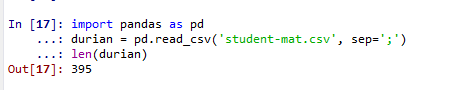
\includegraphics[scale=0.5]{figures/solusi8.png}
\caption{Evaluasi Error}
\label{Eror}
\end{figure}
\end{itemize}
\end{enumerate}